\documentclass[draftmode,eclipse]{preziposters}
\usepackage{brackets,importsreferences,amssymb,marvosym,pifont,lipsum,symsabim,dingbat}
\title{Graphs \& Combinatorial Optimization}
\suptitle{Doctoral course on}
\author{Willem Van Onsem\\KU Leuven\\Department of Computer Science}
\logo{../libtex/sedes.pdf}
\disclaimer{This document is published under the \emph{Beer license revision 42} by \emph{Poul-Henning Kamp}.}
\usetikzlibrary{shapes}
\begin{document}

\def\dma{5 mm};
\def\mid{594.5 mm};
\def\dyl{100.0 mm};
\def\dylm{5.0 mm};
\def\dylma{105.0 mm};
\def\dylhma{65.0 mm};
\def\dylqma{150.0 mm};
\def\dyw{1100.0 mm};
\def\dywb{550.0 mm};
\def\dywt{366.7 mm};
\def\dywq{275.0 mm};
\def\dywu{220.0 mm};
\def\dywh{183.3 mm};

\definecolor{treebg}{rgb}{0.93,0.93,0.69}

\tikzset{ptgtcov/.style={circle,inner sep=0pt,fill=black,minimum size=1.414mm}}

\defgroup[\dma][0][-\dylqma-0.5*\dylma][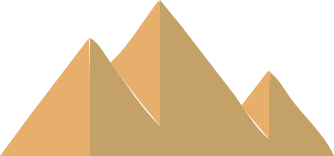
\includegraphics{pyramid.pdf}]{\dywb}{\dylqma}{Basics}{orange}{graph}
\defgroup[\dma][\dywb][-\dylqma-0.5*\dylma][
\includegraphics{walk.pdf}]{\dywb}{\dylqma}{Walks and Reachability}{yellow}{move}
\defgroup[\dma][0][-0.5*\dylma-2*\dylqma][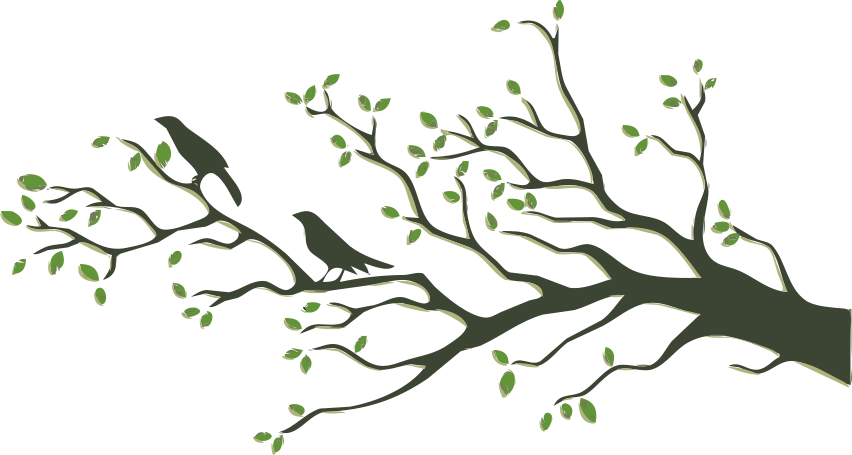
\includegraphics{tree.pdf}]{\dywb}{\dylqma}{Trees}{treebg}{tree}
\defgroup[\dma][\dywb][-0.5*\dylma-2*\dylqma][]{2*\dywt-\dywb}{\dylqma}{Graph coloring}{red}{grcl}
\defgroup[\dma][2*\dywt][-0.5*\dylma-2*\dylqma][]{\dywt}{\dylqma}{Graph families}{purple}{grfa}
\defgroup[\dma][0][-1.5*\dylma-2*\dylqma][]{\dywu}{\dylma}{Legend}{backg}{legen}
\boxfile{definitions.tex}
\def\pztbtc{red}
\boxfile{theorems.tex}
\confile[very thick,open triangle 60-,black!80!white][sloped,above,midway,black]{connections.tex}
% \groupbox{(CCgrph) (CCslfl)}{Vertices and Edges}
\groupbox{(CCgraycod) (CChypergr)}{Bitwise graphs}
\groupbox{(CCcncwl) (CCsubwl)}{Walk operations}
\groupbox{(CCeulert) (CCposttour) (CChamilcyc)}{Special walks}
\groupbox{(CCreach) (CCconn) (CCwkconn) (CCedgcut) (CCvercut) (CCcpn)}{Reachability and components}
\groupbox{(CCprnttree) (CCdscasctree)}{Rooted tree vertex relations}
\groupbox{(CCstree) (CCfronted) (CCtreegrow)}{Tree growing}
\groupbox{(CCmarytree) (CCordtree) (CCbintree)}{Tree variants}
\groupbox{(CCgruni) (CCgrjoin) (CCvdsg) (CCedsg)}{Graph operations}
\end{document}
